\documentclass[11pt,a4paper]{article}
\usepackage[margin=2.5cm]{geometry}
\usepackage{booktabs,tabularx}
\usepackage{graphicx}
\usepackage{amsmath,amssymb}
\usepackage{hyperref}
\usepackage{xcolor}
\usepackage{subcaption}
\graphicspath{{figs/}}

\title{\textbf{Boltzmann Mixture-of-Experts Energy FFN}\\
\large Routing Collapse, Anti-Collapse Strategies, and Expert Specialization}
\author{dolomite-engine experiment series B1--B5, $d{=}768$, ${\approx}422$M params}
\date{2026-04-29}

\begin{document}
\maketitle
\tableofcontents
\newpage

%% ============================================================
\section{Setup}
%% ============================================================

\subsection{Model}

We replace the Energy MLP feedforward in each of 12 EGPT blocks with a
Boltzmann-weighted mixture of $K{=}16$ parallel energy experts:
\begin{equation}
  E_\text{MoE}(h) = \tau \log \sum_{i=1}^{K} \exp\!\bigl(E_i(h)/\tau\bigr),
  \qquad
  E_i(h) = \varphi(W_1^{(i)}h)^\top (W_2^{(i)}h),
  \label{eq:energy}
\end{equation}
where $\varphi$ is GELU and $\tau{=}1$ (temperature).  The gradient, used as
the FFN output block, is the Boltzmann-weighted average of per-expert gradients:
\begin{equation}
  \frac{\partial E_\text{MoE}}{\partial h}
  = \sum_{i=1}^K p_i(h)\,\frac{\partial E_i}{\partial h},
  \qquad
  p_i(h) = \frac{\exp(E_i(h)/\tau)}{\sum_j \exp(E_j(h)/\tau)}.
  \label{eq:grad}
\end{equation}
The routing energy $E_i$ is computed as $h \cdot \text{term}_1^{(i)}$ where
$\text{term}_1^{(i)} = \varphi(W_1^{(i)}h)^\top W_2^{(i)}$ is the first
gradient term (contracting only the first term avoids a spurious Hessian
contribution from the full gradient).

\paragraph{Deep EGPT.}
B1--B5 are \emph{deep} EGPT models: 12 \emph{distinct} blocks each with
independent weights, not a single block looped.
Recurrent variants (V58, V63) loop one block multiple times and have far fewer
non-embedding parameters.

\paragraph{Iso-parameter design and architecture imbalance.}
Each of the 16 experts has intermediate size 1024 (total $16{\times}1024{=}16\,384$),
identical total FLOPs and parameters to one Energy\_MLP of the same total size.
However, the resulting model is severely \emph{FFN-heavy}: 302M of 407M
non-embedding parameters are in the MoE FFN (FFN:Attn $\approx$\,21:1),
compared to $\approx$\,2--3:1 for the GPT and EGPT baselines.
This architectural imbalance is the primary reason MoE underperforms the baselines.
Table~\ref{tab:params} shows the breakdown.

\begin{table}[ht]
\centering
\caption{Parameter breakdown.  All counts in millions.  FFN:Attn = ratio of FFN
  to attention parameters (excluding embedding and projections).}
\label{tab:params}
\small
\resizebox{\textwidth}{!}{\begin{tabular}{lrrrrrr}
\toprule
Model & Total & Embed & Attn & FFN/MoE & Proj & FFN:Attn \\
\midrule
V1 EGPT ($d{=}768$, 12 layers)     & 143 & 77 & 14 &  38 & 14 &  2.7 \\
B1--B5 (BoltzMoE, $d{=}768$) & 407 & 77 & 14 & 302 & 14 & 21.3 \\
V9 GPT ($d{=}1024$, 24 layers) & 354 & 103 & 75 & 151 & 0 & 2.0 \\
V1-400M EGPT ($d{=}1024$, 24 layers) & 354 & 103 & 50 & 151 & 50 & 3.0 \\
V58 EGPT recurrent ($d{=}1024$, 1 block$\times$24) & 113 & 103 & 2 & 6 & 2 & 2.7 \\
\bottomrule
\end{tabular}}
\end{table}

\subsection{Anti-collapse strategies}

\begin{table}[h]
\centering
\caption{Experimental variants.}
\label{tab:variants}
\begin{tabular}{llll}
\toprule
Run & Repulsion $\lambda$ & Dropout & Weight decay \\
\midrule
B1 & --- & 0 & 0.1 \\
B2 & 0.01 & 0 & 0.1 \\
B3 & 0.01 & 0.1 & 0.3 \\
B4 & 0.1  & 0   & 0.1 \\
B5 & 0.1  & 0.1 & 0.3 \\
\bottomrule
\end{tabular}
\end{table}

\noindent\textbf{Stochastic contrastive repulsion.}
At each training step, $K_r{=}4$ random expert pairs $(i,j)$ are sampled and
their output cosine similarity is penalised:
$\mathcal{L}_\text{rep} = \lambda\,\mathbb{E}_{(i,j)}[\cos(g_i,g_j)]$
where $g_i = \partial E_i/\partial h$.

\subsection{Training}
All runs: 30k steps, cosine LR from 2e-3 with 2k warmup, 7.86B tokens,
4 GPUs, \texttt{bf16}, \texttt{torch.compile}, FSDP stage~2.

%% ============================================================
\section{Routing collapse analysis}
%% ============================================================

\subsection{Metrics}

We track three complementary metrics, each capturing a different aspect of routing:
\begin{itemize}
  \item $\hat{K} = \exp(\mathbb{E}_h[\mathcal{H}(p(\cdot|h))])$ ---
        \textbf{effective number of experts} per token, exponentiated per-token entropy.
        $\hat{K}{=}1$: each token routes entirely to one expert (hard routing).
        $\hat{K}{=}16$: perfectly uniform.
  \item $\ell_\text{max}$ --- fraction of tokens in a batch for which a given expert
        wins the argmax.  Uniform baseline: $1/K{=}0.0625$.
  \item $n_\text{dom}$ --- number of distinct experts that are the argmax for
        at least one token across the batch.
\end{itemize}

\paragraph{Interpretation of $n_\text{dom}{=}16$ on WandB.}
The WandB metric shows $n_\text{dom}{=}16$ throughout training because,
\emph{across a full batch of} ${\sim}16\,000$ tokens, all 16 experts win at
least one token.  This does \emph{not} mean equal contribution: per-token
routing is near-one-hot ($\hat{K}{\approx}1$), i.e.\ each token decisively
picks one expert, but different tokens pick different experts.
The relevant collapse metric is $\ell_\text{max}$ (how concentrated the load
is) and the per-question-category argmax analysis (Section~\ref{sec:spec}).

\subsection{Results}

\begin{figure}[ht]
  \centering
  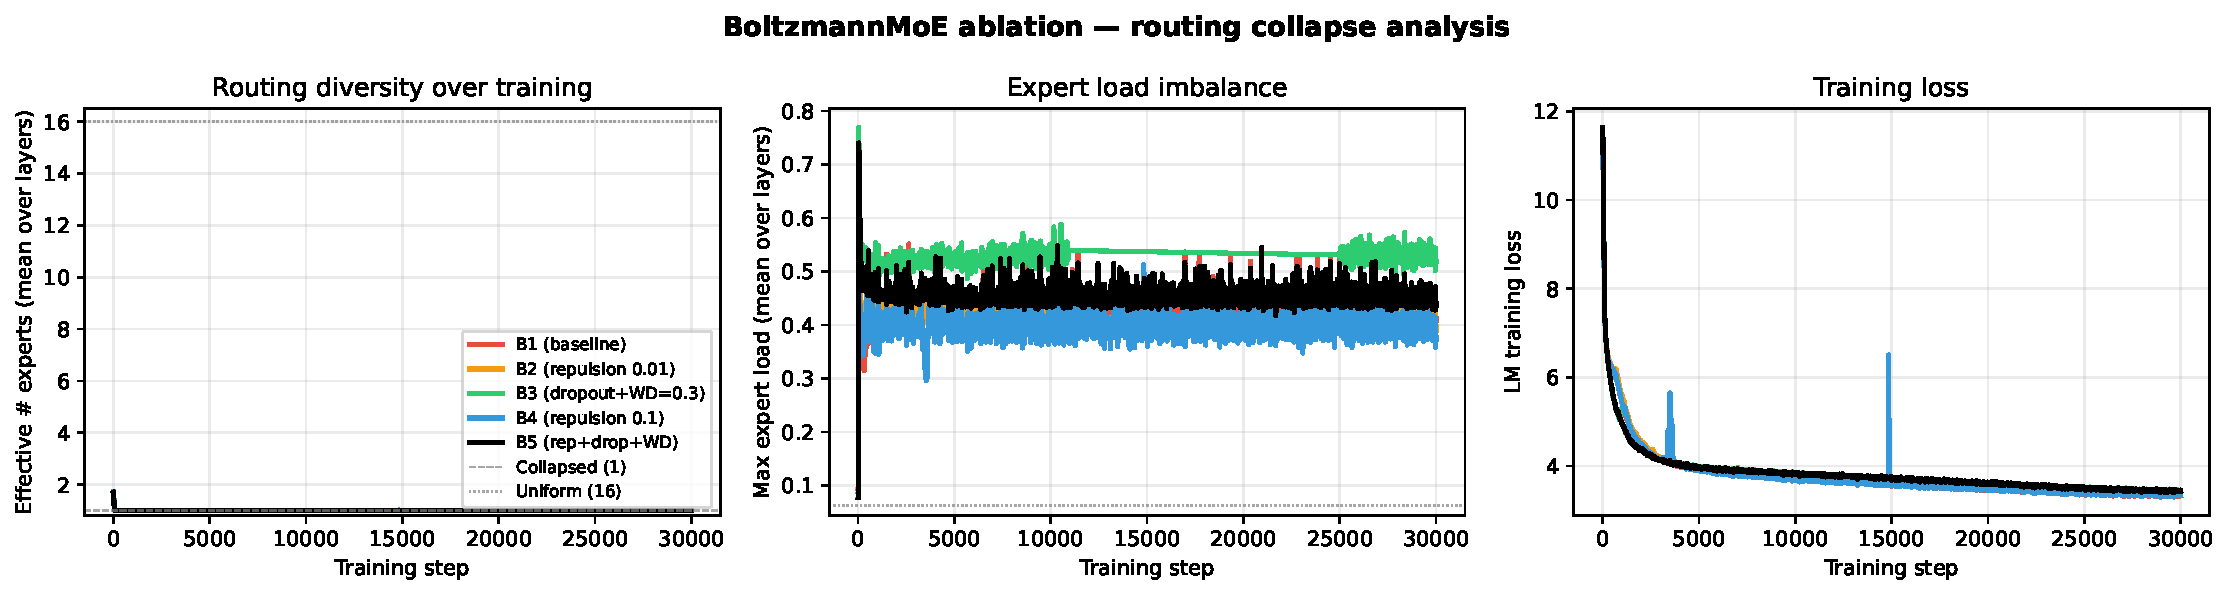
\includegraphics[width=\textwidth]{boltz_routing_collapse_comparison.pdf}
  \caption{Routing evolution over training.
    \textbf{Left}: effective number of experts $\hat{K}$ (layers 8--11 mean).
    \textbf{Centre}: max expert load $\ell_\text{max}$.
    \textbf{Right}: LM training loss.
    All runs develop hard per-token routing ($\hat{K}\approx 1$) by step~500.
    B4 ($\lambda{=}0.1$) achieves the best load balance at comparable steps.
    B3 (dropout+WD) worsens load balance and deep-layer expert diversity.}
  \label{fig:routing_evolution}
\end{figure}

\begin{table}[ht]
\centering
\caption{Routing metrics at step 30k, all runs complete (layers 8--11 mean).
  $\hat{K}{=}1$ = hard routing; $\hat{K}{=}16$ = uniform; uniform $\ell_\text{max}$ = 0.063.}
\label{tab:routing}
\begin{tabular}{lrrrr}
\toprule
Model & $\hat{K}$ & $\ell_\text{max}$ & $n_\text{dom}$ & LM loss \\
\midrule
B1 (no reg.)            & 1.005 & 0.409 & 14.75 & 3.330 \\
B2 ($\lambda_r{=}0.01$) & 1.004 & 0.391 & 13.50 & 3.338 \\
B3 (drop.+WD=0.3)       & 1.009 & 0.519 &  9.75 & 3.433 \\
B4 ($\lambda_r{=}0.1$)  & 1.004 & \textbf{0.373} & 14.00 & 3.336 \\
B5 (rep+drop+WD)        & 1.009 & 0.436 & 14.00 & 3.432 \\
\bottomrule
\end{tabular}
\end{table}

Key observations:
\begin{itemize}
  \item Hard routing ($\hat{K}{\approx}1$) emerges universally by step~500.
  \item B4 (repulsion only, $\lambda{=}0.1$) achieves the best load balance
        ($\ell_\text{max}{=}0.39$) with the same LM loss as B2.
  \item B3 (dropout + WD=0.3) \emph{worsens} both load balance and
        deep-layer diversity --- WD drives weights toward zero, reducing
        discriminability and amplifying imbalance.
  \item The stochastic repulsion signal scales well: $\lambda{=}0.1$
        (B4) is clearly better than $\lambda{=}0.01$ (B2) with no loss penalty.
\end{itemize}

%% ============================================================
\section{Benchmark results}
%% ============================================================

\begin{table}[ht]
\centering
\caption{Zero-shot benchmark results (30k steps, 7.86B tokens).
  Avg = 9-task mean (acc\_norm where applicable).
  \dag{} V63 result pending (20k/30k steps).}
\label{tab:benchmarks}
\small
\resizebox{\textwidth}{!}{\begin{tabular}{lrrrrrrrrrrrr}
\toprule
 & Params & ARC-C & ARC-E & BoolQ & COPA & HellaS & OB-QA & PIQA & SciQ & Wino & \textbf{Avg} & WikiPPL \\
\midrule
\multicolumn{13}{l}{\textit{Baselines}} \\
V9 GPT $d{=}1024$        & 354M & .287 & .545 & .622 & .740 & .457 & .344 & .718 & .817 & .534 & \textbf{.563} & \textbf{29.8} \\
V1-400M EGPT $d{=}1024$  & 354M & .245 & .497 & .628 & .720 & .386 & .318 & .683 & .775 & .513 & .530 & 38.6 \\
V58 EGPT 1$\times$24 recur. & 113M & .230 & .414 & .563 & .620 & .292 & .278 & .644 & .649 & .504 & .466 & 65.7 \\
V1 EGPT ($d{=}768$, 12 layers) & 143M & .236 & .446 & .611 & .640 & .308 & .292 & .622 & .666 & .507 & \textbf{.481} & 47.7 \\
V63 EGPT 1$\times$12 $d{=}$1408 & --- & \multicolumn{10}{c}{\emph{pending (20k/30k steps)}} & --- \\
\midrule
\multicolumn{13}{l}{\textit{BoltzmannMoE (deep EGPT, $d{=}768$, 16 experts$\times$1024, $\approx$422M)}} \\
B1 (no reg.)      & 407M & .221 & .429 & .594 & \textbf{.660} & .305 & .298 & .619 & .637 & .504 & .474 & 51.9 \\
B2 (rep 0.01)     & 407M & .233 & .417 & .585 & .590 & .303 & .268 & .627 & .638 & .500 & .462 & 52.5 \\
B3 (drop+WD=0.3)  & 407M & .246 & .413 & .461 & .620 & .297 & .274 & .616 & .616 & .509 & .450 & 58.0 \\
B4 (rep 0.1)      & 407M & .227 & .431 & .567 & .620 & .307 & .282 & .625 & .631 & .499 & .466 & 51.9 \\
B5 (rep+drop+WD)  & 407M & .228 & .419 & .603 & .620 & .291 & .292 & .625 & .658 & .505 & .471 & 58.7 \\
\bottomrule
\end{tabular}}
\end{table}

\noindent\textbf{The MoE does not beat the baselines.}
V9 GPT (354M, $d{=}1024$) achieves 0.563 avg vs.\ 0.474 for the best MoE (B1),
and V1-400M EGPT achieves 0.530 --- both at fewer total parameters.
WikiText PPL tells the same story: GPT 29.8, EGPT 38.6, vs.\ 51.9--58.7 for MoE.

The root cause is the architecture imbalance (Table~\ref{tab:params}):
the MoE allocates 302M of 407M parameters to the FFN (21:1 FFN:Attn),
leaving only 14M for attention.  In contrast, both baselines have FFN:Attn
$\approx$\,2--3:1.  Capacity collapses to only 2--3 experts, so the MoE
effectively behaves as a 2-expert ensemble of small FFNs, losing the benefit
of the MoE capacity entirely.

The exception is COPA (commonsense causal reasoning), where B1 scores 0.660
vs.\ V9's 0.740 but still outperforms V58 (0.620) and all regularised MoE
variants, consistent with COPA's unique routing cluster (Section~\ref{sec:spec}).

\noindent\textbf{Within the MoE ablation:}
B1 (no regularisation) is the best MoE variant (0.474, PPL 51.9).
B4 (repulsion $\lambda{=}0.1$) improves load balance ($\ell_\text{max}$ 0.373
vs.\ 0.409) at marginal accuracy cost (0.466).
Dropout+WD variants (B3, B5) consistently hurt both accuracy and PPL.

%% ============================================================
\section{Expert specialization analysis}
\label{sec:spec}
%% ============================================================

\subsection{Setup}
We ran inference with B1 and B5 on 60 samples per category from:
MMLU (5 subject groups), BoolQ, COPA, and GSM8k.
For each input, per-layer Boltzmann routing weights $p_i(h)$ were captured
by hooking into the forward pass.  Routing vectors were averaged over sequence
tokens per sample.

\subsection{Key finding: semantic expert specialization with load concentration}

Despite 16 experts, only \textbf{2--3 experts handle all question types}.
This is not random: specific experts consistently dominate specific semantic categories.

\begin{table}[ht]
\centering
\caption{Expert argmax analysis by category (mean over all layers).
  ``Active'' = number of distinct experts that ever win argmax.
  ``Top expert'' = expert index winning the most samples and its fraction.}
\label{tab:specialization}
\begin{tabular}{lcccc}
\toprule
Category & \multicolumn{2}{c}{B1} & \multicolumn{2}{c}{B5} \\
\cmidrule(lr){2-3}\cmidrule(lr){4-5}
 & Active & Top (\%) & Active & Top (\%) \\
\midrule
MMLU-STEM       & 2 & \#13 (66\%) & 3 & \#3 (75\%) \\
MMLU-Humanities & 2 & \#3  (75\%) & 2 & \#3 (53\%) \\
MMLU-Social     & 2 & \#3  (92\%) & 3 & \#3 (56\%) \\
MMLU-Medical    & 2 & \#13 (75\%) & 2 & \#3 (83\%) \\
MMLU-Logic      & 2 & \#3  (60\%) & 3 & \#3 (58\%) \\
BoolQ           & 2 & \#13 (78\%) & 3 & \#11 (92\%) \\
COPA            & 2 & \#13 (70\%) & 2 & \#11 (88\%) \\
GSM8k           & 2 & \#13 (93\%) & 3 & \#3  (48\%) \\
\midrule
\multicolumn{5}{l}{\textit{B1 pattern: Expert \#13 = factual/task; Expert \#3 = reasoning/language}} \\
\multicolumn{5}{l}{\textit{B5 pattern: Expert \#3 = general; Expert \#11 = commonsense reasoning}} \\
\bottomrule
\end{tabular}
\end{table}

\paragraph{B1 routing structure.}
Two experts dominate: \textbf{Expert \#13} handles STEM, Medical, BoolQ, COPA,
and GSM8k (66--93\% of samples); \textbf{Expert \#3} handles Humanities, Social,
and Logic (60--92\%).  This suggests a \emph{factual/task-oriented} vs.\
\emph{language/reasoning} split.

\paragraph{B5 routing structure.}
Dropout+WD reshuffled the split: \textbf{Expert \#3} now dominates most MMLU
categories, while \textbf{Expert \#11} takes over commonsense reasoning tasks
(BoolQ 92\%, COPA 88\%).  The specialization is clearer for commonsense tasks
but less differentiated across MMLU subjects.

\subsection{Figures: expert load and routing heatmap}

\begin{figure}[ht]
  \centering
  \begin{subfigure}[b]{\textwidth}
    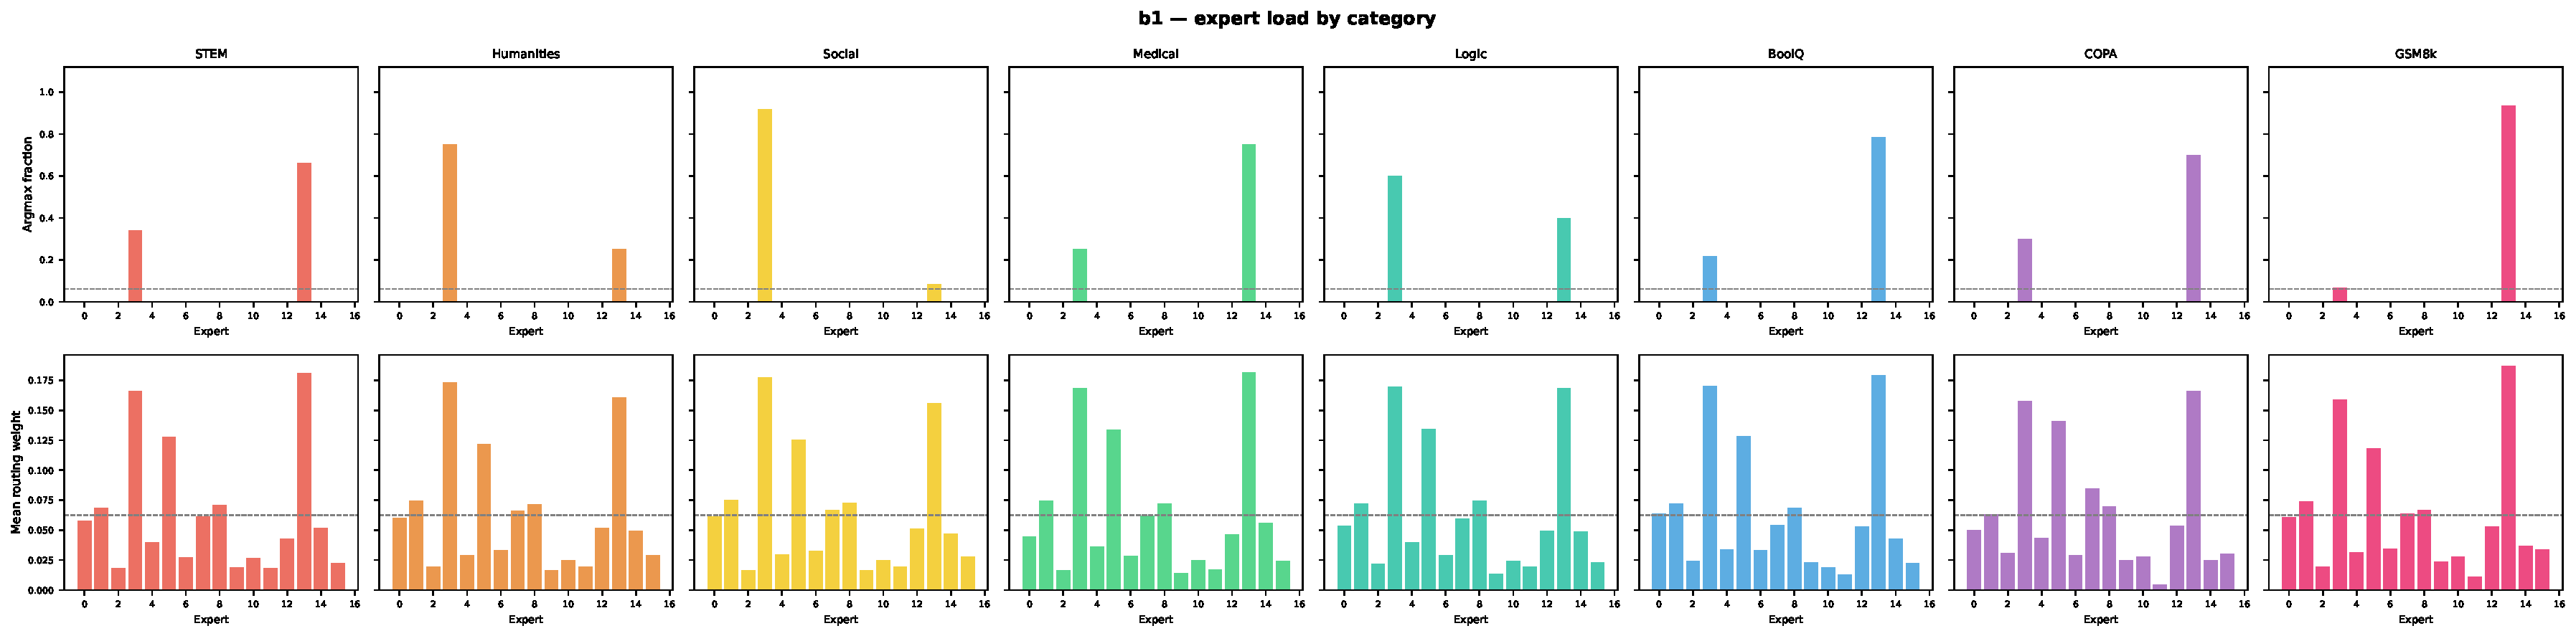
\includegraphics[width=\textwidth]{expert_load_b1.pdf}
    \caption{B1 (no regularisation)}
  \end{subfigure}
  \vspace{1em}
  \begin{subfigure}[b]{\textwidth}
    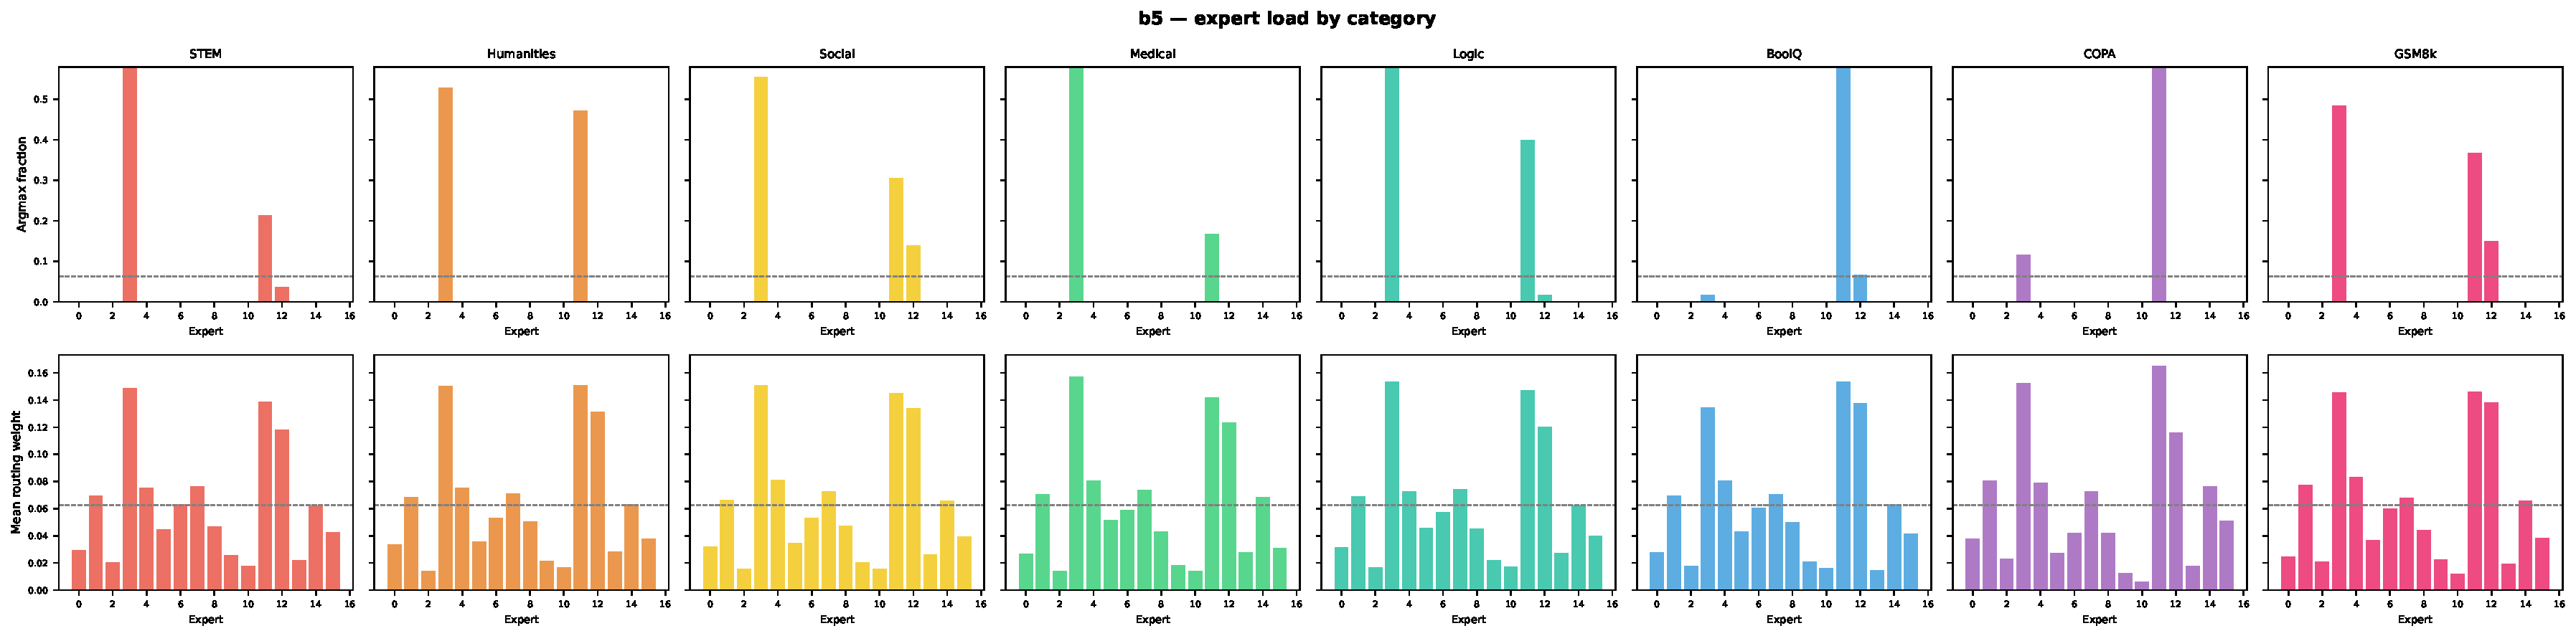
\includegraphics[width=\textwidth]{expert_load_b5.pdf}
    \caption{B5 (rep\,0.1 + dropout + WD=0.3)}
  \end{subfigure}
  \caption{Expert argmax fraction (top row) and mean routing weight (bottom row) per
    category.  B1 shows a clear two-expert structure; B5 shows Expert \#3
    dominating MMLU with Expert \#11 specialising on commonsense tasks (BoolQ/COPA).}
  \label{fig:load}
\end{figure}

\begin{figure}[ht]
  \centering
  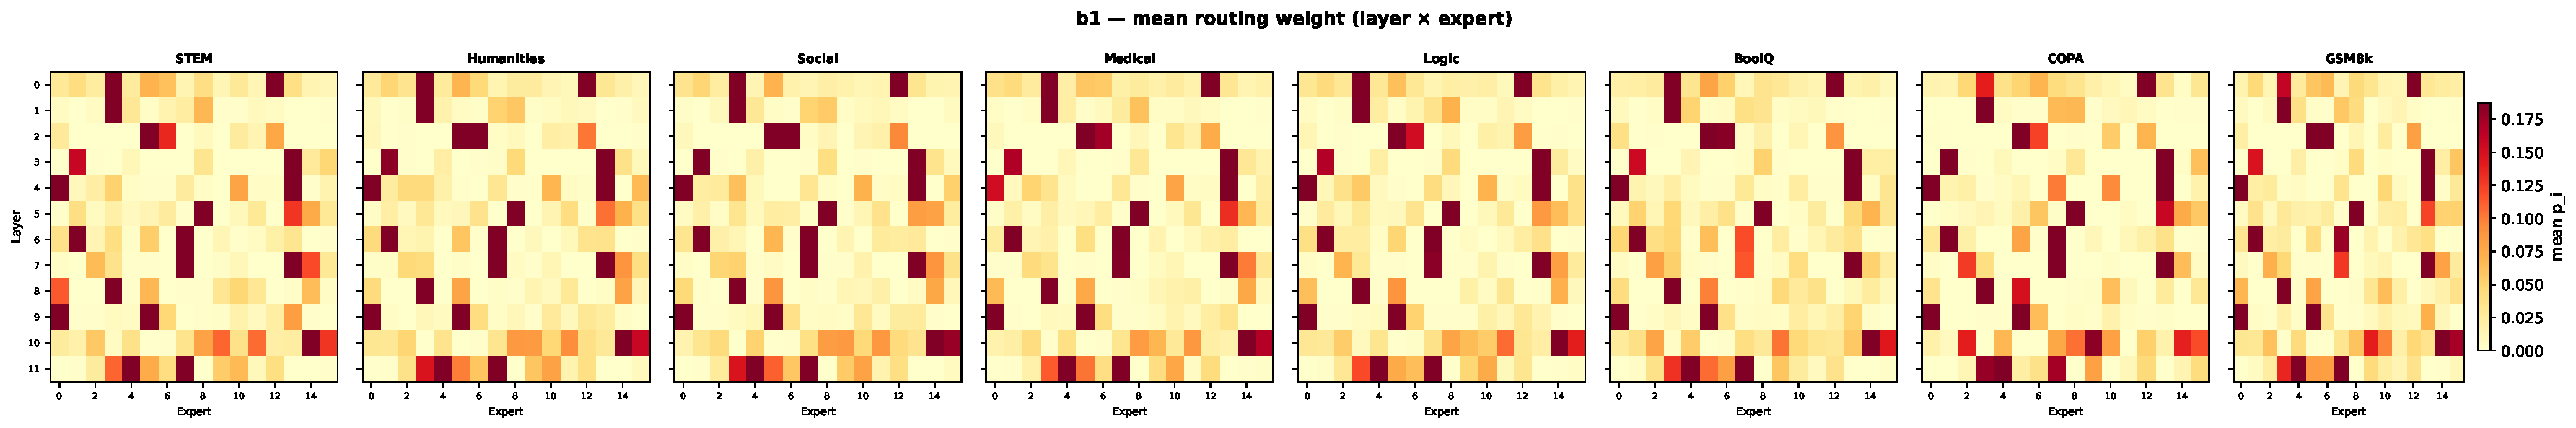
\includegraphics[width=\textwidth]{expert_routing_heatmap_b1.pdf}
  \caption{B1 per-layer routing heatmap (layer $\times$ expert, mean weight).
    Expert \#13 activates strongly in early layers for task-oriented inputs;
    Expert \#3 activates in middle-to-late layers for language/reasoning inputs.}
  \label{fig:heatmap}
\end{figure}

\subsection{Mean-centred PCA: residual routing patterns}
\label{sec:pca_deep}

Raw routing vectors are dominated by the 2--3 globally active experts, making
category differences invisible.  Subtracting the global mean routing vector reveals
the \emph{residual} pattern: which experts a category uses \emph{relative to the
average}.

\begin{figure}[ht]
  \centering
  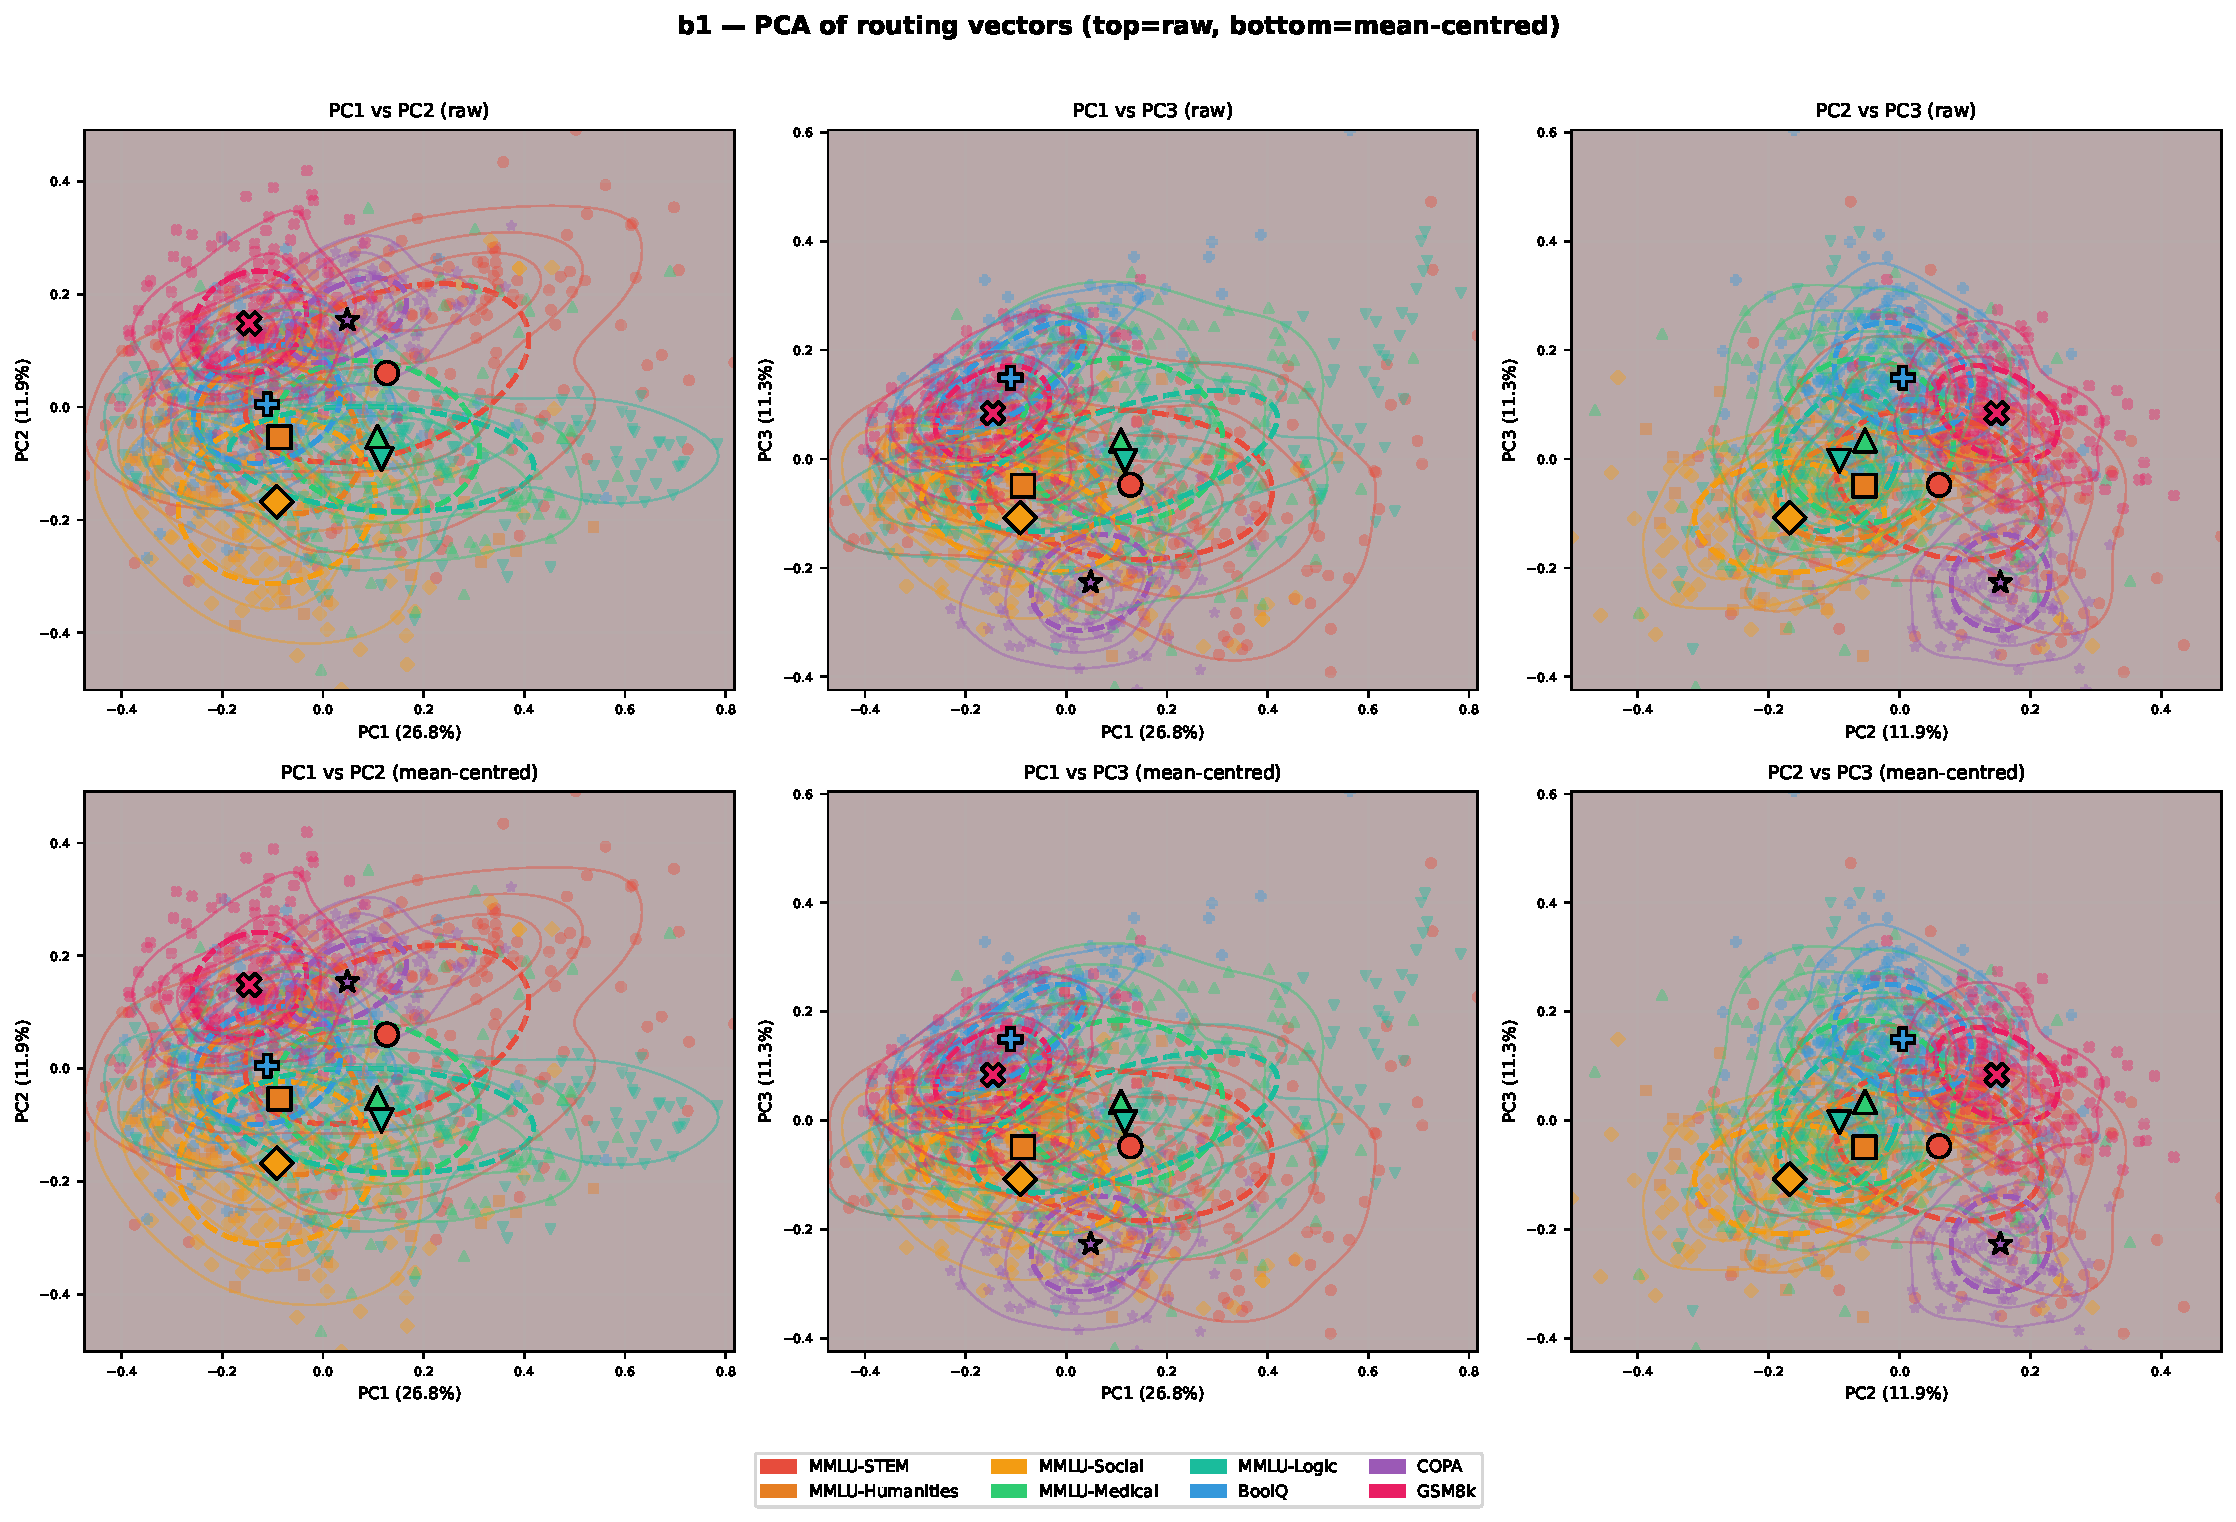
\includegraphics[width=\textwidth]{expert_pca_deep_b1.pdf}
  \caption{B1 routing PCA: raw (top row) vs.\ mean-centred (bottom row), with
    PC1/2, PC1/3, PC2/3.  KDE contours show per-category density;
    large markers are centroids; dashed ellipses show $1\sigma$ spread.
    After mean-centering, COPA is completely isolated from all other categories
    across all PC pairs.  GSM8k, MMLU-STEM, Medical, and BoolQ occupy
    distinct PCA regions; MMLU-Humanities/Social/Logic cluster together.}
  \label{fig:pca_deep_b1}
\end{figure}

\begin{figure}[ht]
  \centering
  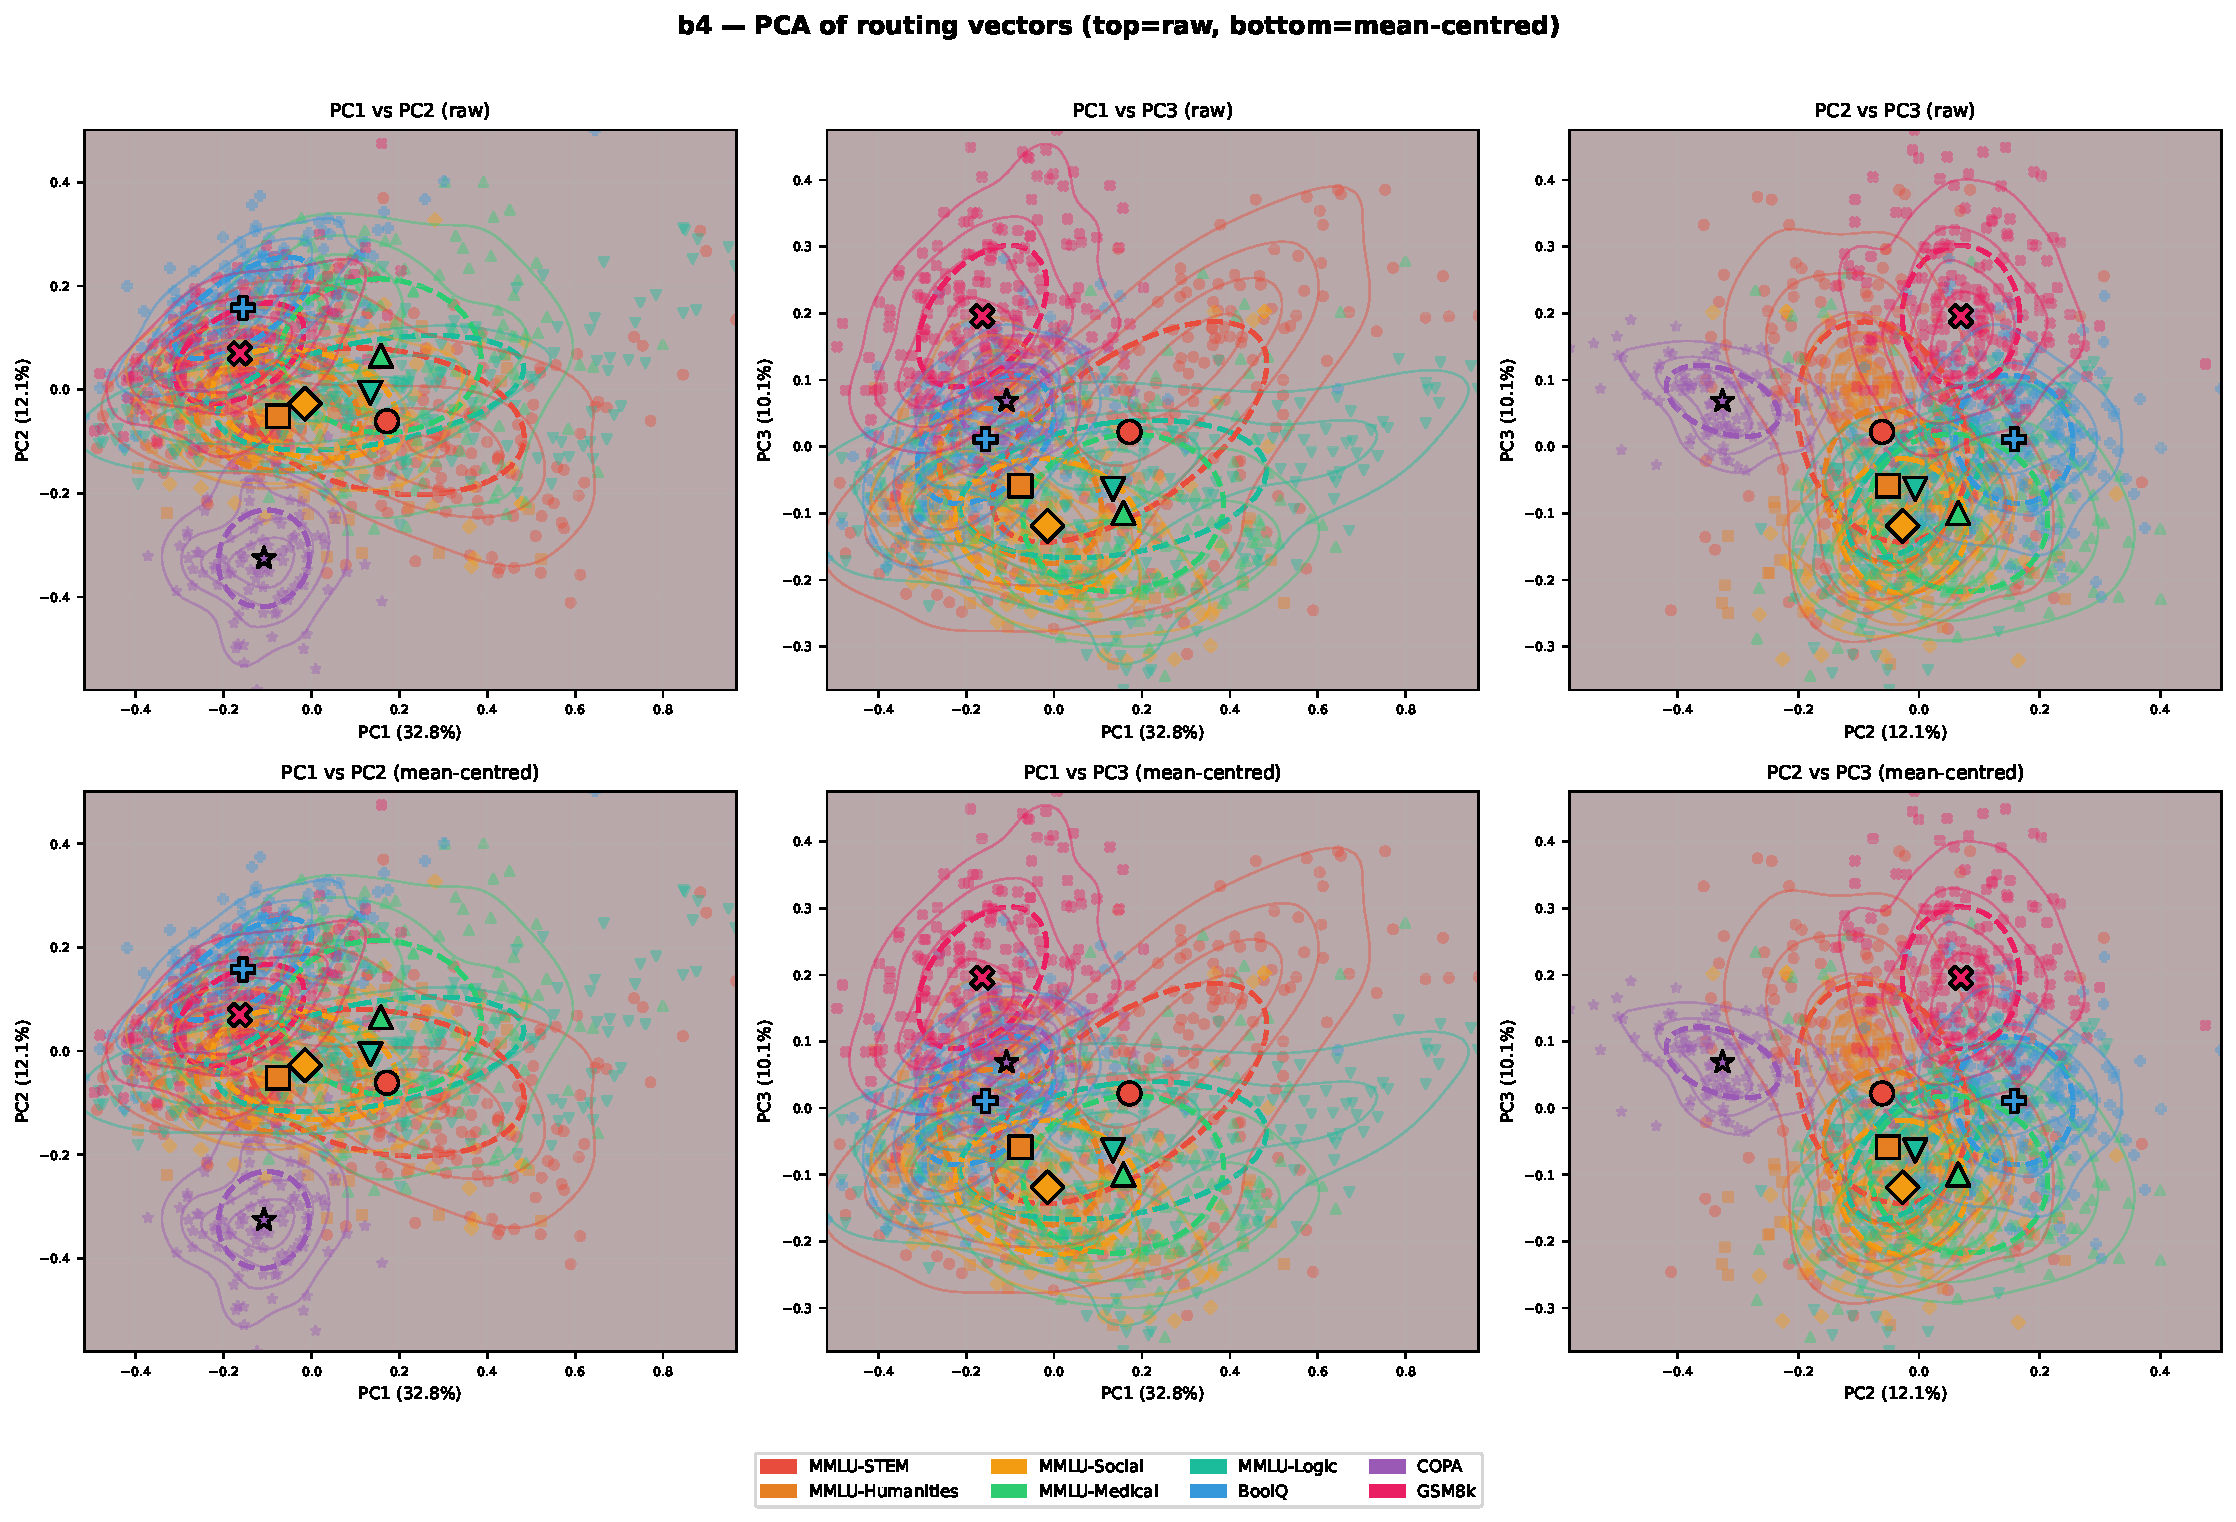
\includegraphics[width=\textwidth]{expert_pca_deep_b4.pdf}
  \caption{B4 (rep\,0.1) routing PCA.  Repulsion increases COPA's isolation
    further; the MMLU cluster is more diffuse, suggesting experts spread
    their activations more evenly across knowledge domains.}
  \label{fig:pca_deep_b4}
\end{figure}

\begin{figure}[ht]
  \centering
  \begin{subfigure}[b]{\textwidth}
    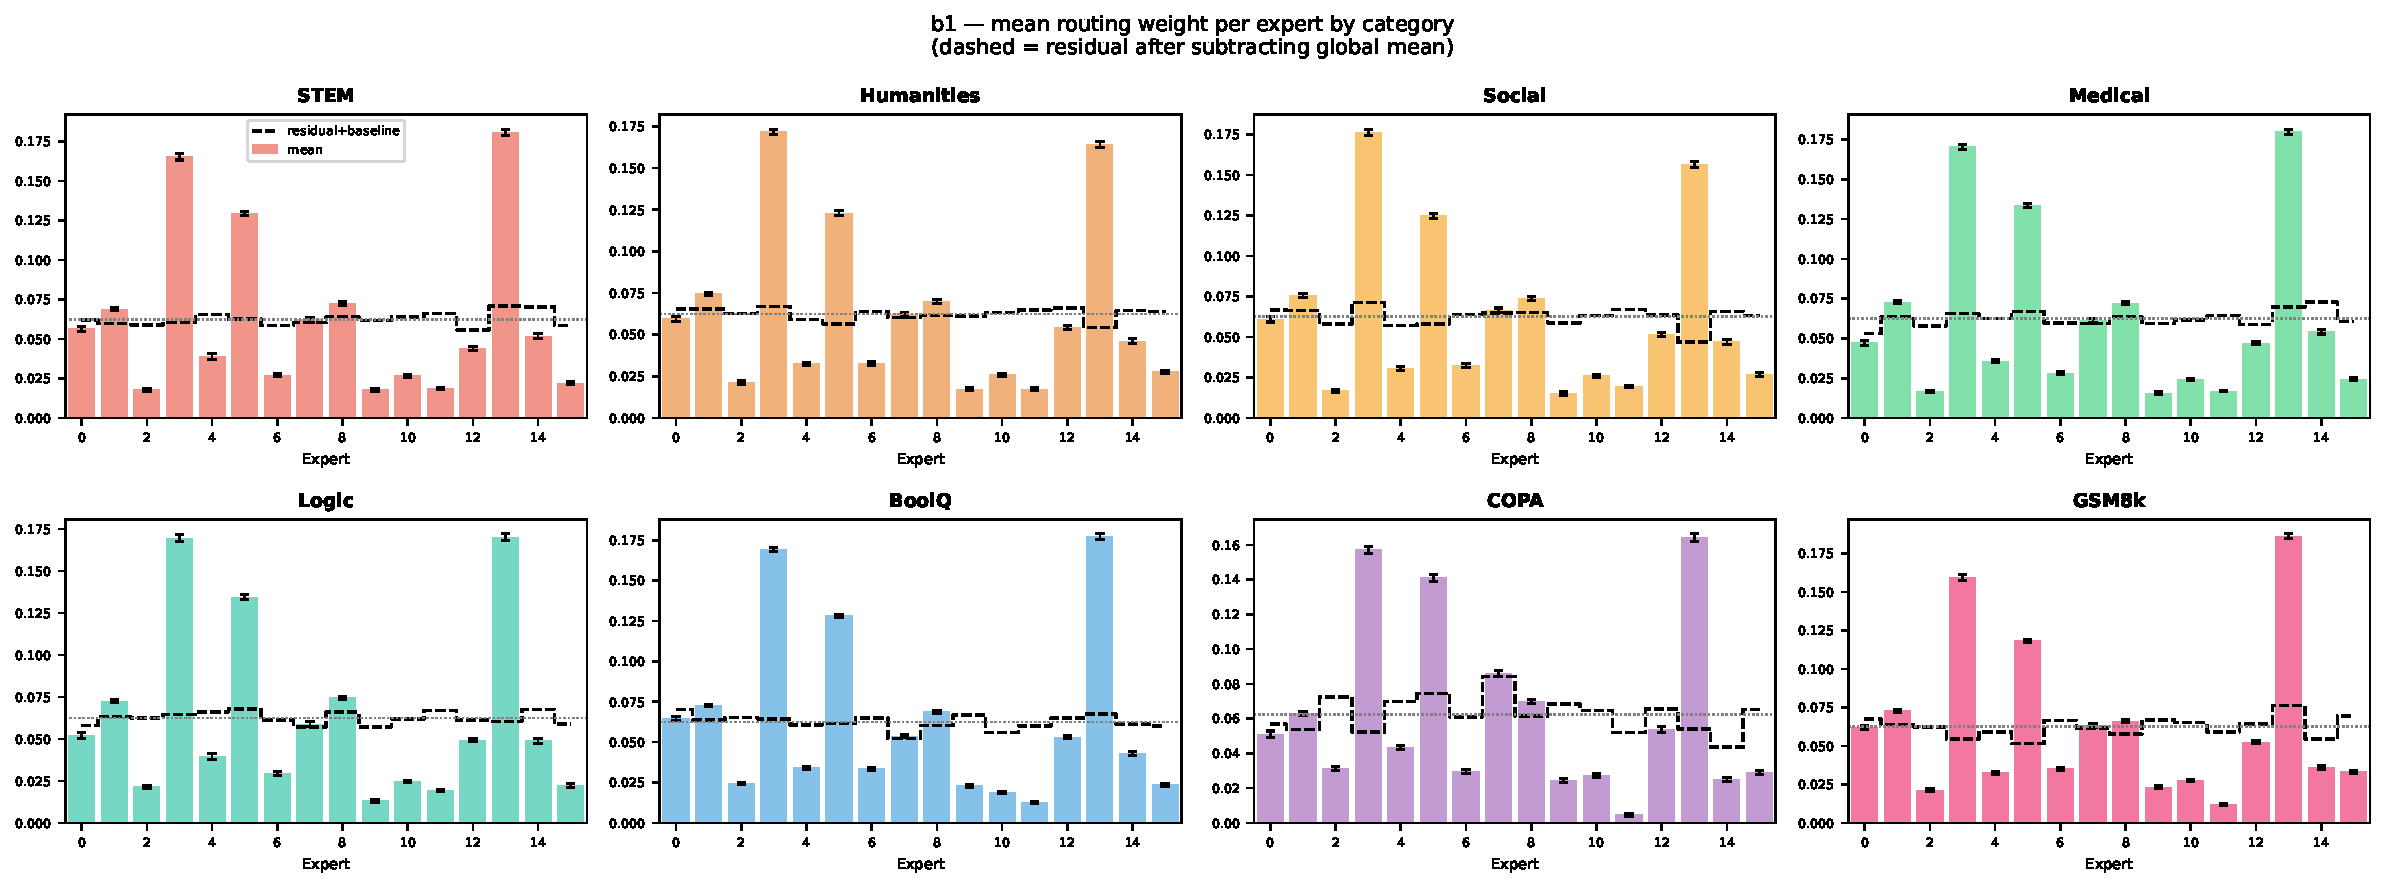
\includegraphics[width=\textwidth]{expert_profiles_b1.pdf}
    \caption{B1: mean $\pm$ 95\,\% CI routing weight per expert.
      Dashed line = residual after subtracting global mean.}
  \end{subfigure}
  \vspace{0.5em}
  \begin{subfigure}[b]{\textwidth}
    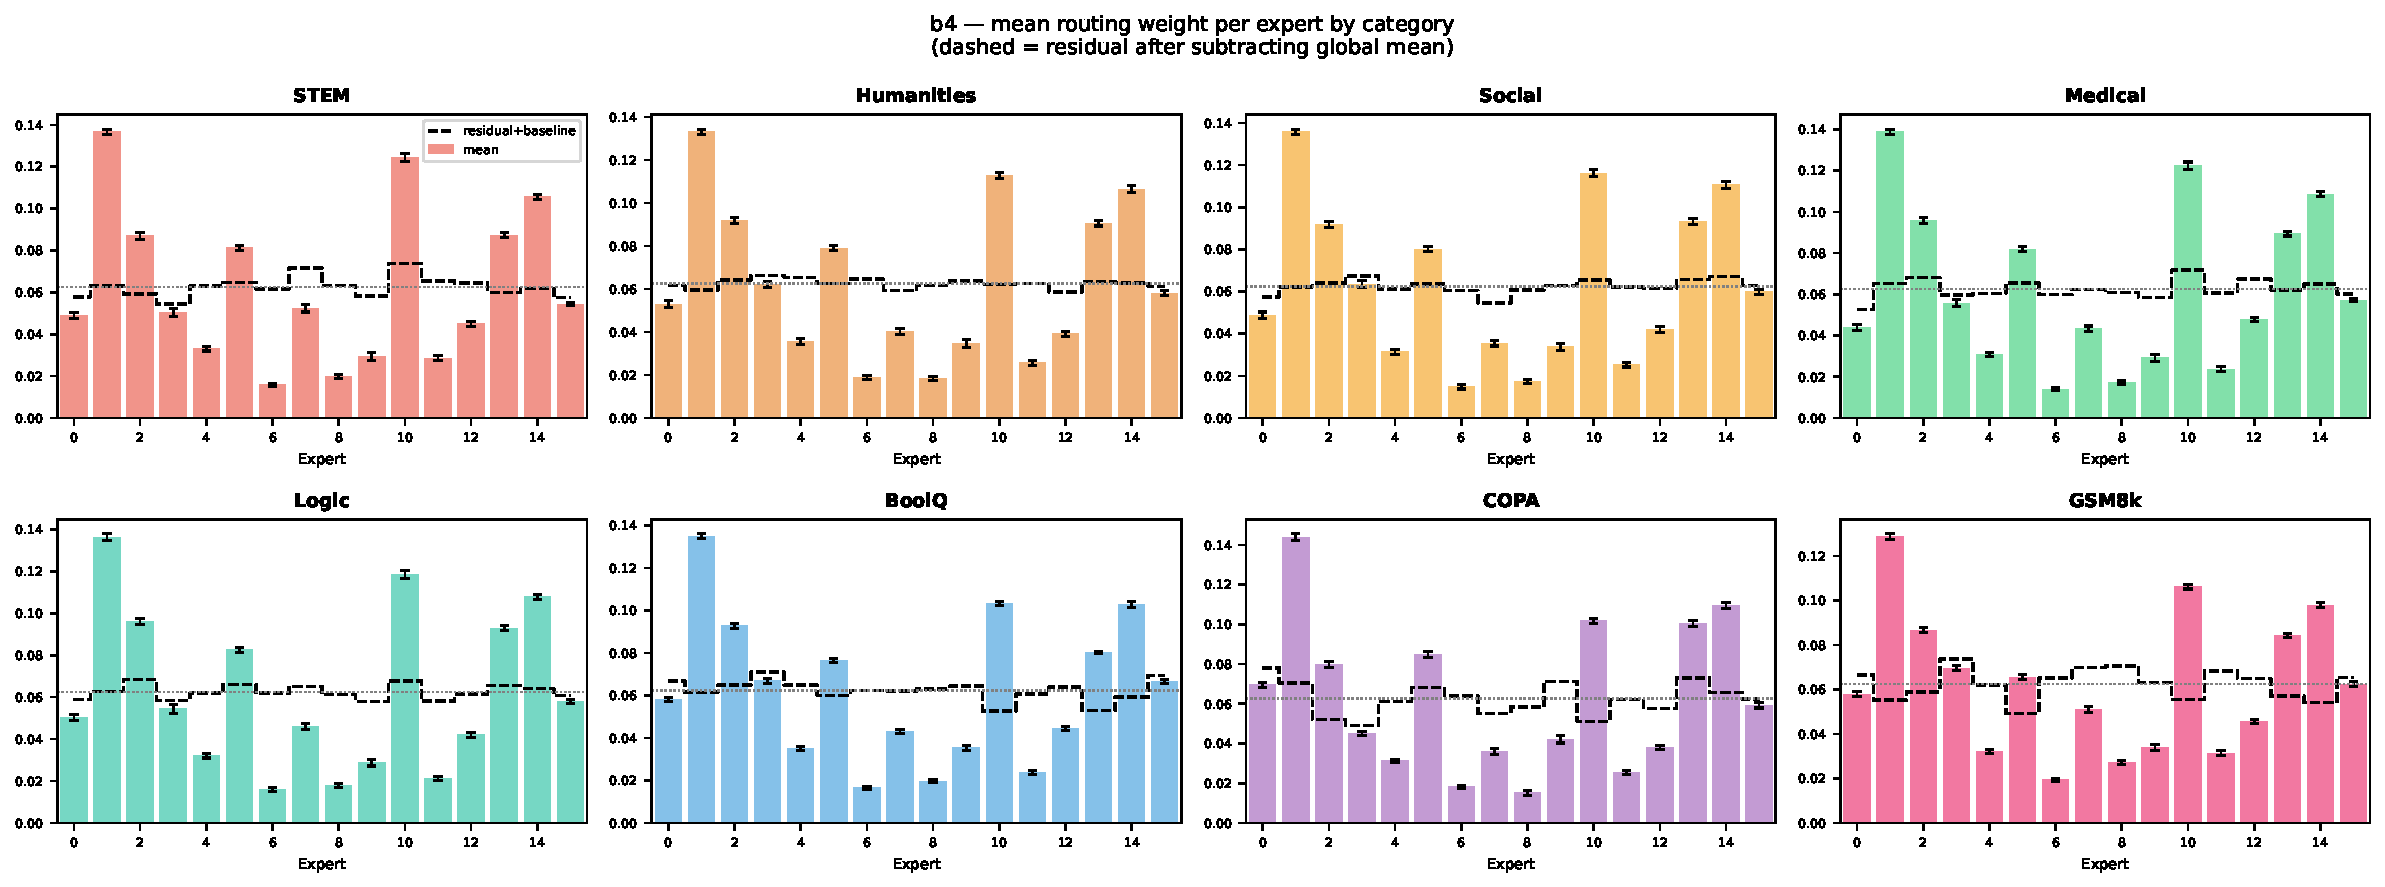
\includegraphics[width=\textwidth]{expert_profiles_b4.pdf}
    \caption{B4 (rep\,0.1): same layout.  Repulsion spreads activation
      more evenly; the residual patterns are smaller but persist.}
  \end{subfigure}
  \caption{Per-category routing profiles.  Despite overall dominance by 2--3 experts,
    each category has a distinct residual fingerprint in the remaining experts.}
  \label{fig:profiles}
\end{figure}

\subsection{Pairwise separation: Mahalanobis distance and Cohen's $d$}
\label{sec:separation}

We quantify routing separation between categories using two metrics computed in
an 8-dimensional mean-centred PCA space:
\begin{itemize}
  \item \textbf{Mahalanobis distance}: $d_M(i,j) = \sqrt{(\mu_i-\mu_j)^\top
    \hat\Sigma_p^{-1}(\mu_i-\mu_j)}$ where $\hat\Sigma_p$ is the Ledoit--Wolf
    pooled covariance across all categories.
  \item \textbf{Cohen's $d$}: $d_C(i,j) = \|\mu_i-\mu_j\|_2\,/\,(\sigma_i+\sigma_j)$
    where $\sigma_k$ is the mean per-PC within-class std.
\end{itemize}

\begin{table}[ht]
\centering
\small
\caption{Pairwise Mahalanobis distance between category routing centroids (B1,
  8-D mean-centred PCA space, Ledoit--Wolf pooled covariance).
  COPA is the clear outlier ($d_M > 7$ from all others vs.\ $1.2$--$4.1$ within
  the rest).}
\label{tab:mahal_b1}
\resizebox{\textwidth}{!}{\begin{tabular}{lrrrrrrrr}
\toprule
 & STEM & Hum & Soc & Med & Logic & BoolQ & COPA & GSM8k \\
\midrule
STEM   &  0.00 &  1.74 &  2.34 &  1.52 &  1.85 &  2.97 &  \textbf{7.26} &  3.37 \\
Hum    &  1.74 &  0.00 &  1.20 &  2.11 &  1.44 &  2.42 &  \textbf{7.28} &  3.25 \\
Soc    &  2.34 &  1.20 &  0.00 &  2.43 &  1.89 &  3.13 &  \textbf{7.70} &  4.08 \\
Med    &  1.52 &  2.11 &  2.43 &  0.00 &  1.99 &  3.31 &  \textbf{7.77} &  3.51 \\
Logic  &  1.85 &  1.44 &  1.89 &  1.99 &  0.00 &  2.99 &  \textbf{7.13} &  4.04 \\
BoolQ  &  2.97 &  2.42 &  3.13 &  3.31 &  2.99 &  0.00 &  \textbf{7.66} &  2.80 \\
COPA   &  7.26 &  7.28 &  7.70 &  7.77 &  7.13 &  7.66 &  0.00 &  7.03 \\
GSM8k  &  3.37 &  3.25 &  4.08 &  3.51 &  4.04 &  2.80 &  \textbf{7.03} &  0.00 \\
\bottomrule
\end{tabular}}
\end{table}

\begin{table}[ht]
\centering
\small
\caption{Pairwise Mahalanobis distance (B4, rep\,$\lambda{=}0.1$).
  COPA isolation increases further ($d_M > 8$) and within-MMLU distances
  grow slightly, suggesting repulsion promotes broader expert specialisation.}
\label{tab:mahal_b4}
\resizebox{\textwidth}{!}{\begin{tabular}{lrrrrrrrr}
\toprule
 & STEM & Hum & Soc & Med & Logic & BoolQ & COPA & GSM8k \\
\midrule
STEM   &  0.00 &  2.03 &  2.17 &  1.68 &  1.67 &  3.00 &  \textbf{8.64} &  3.52 \\
Hum    &  2.03 &  0.00 &  0.98 &  1.86 &  1.34 &  2.68 &  \textbf{8.12} &  3.20 \\
Soc    &  2.17 &  0.98 &  0.00 &  1.46 &  1.64 &  2.79 &  \textbf{8.23} &  3.49 \\
Med    &  1.68 &  1.86 &  1.46 &  0.00 &  1.44 &  2.52 &  \textbf{8.76} &  3.70 \\
Logic  &  1.67 &  1.34 &  1.64 &  1.44 &  0.00 &  2.99 &  \textbf{8.53} &  3.89 \\
BoolQ  &  3.00 &  2.68 &  2.79 &  2.52 &  2.99 &  0.00 &  \textbf{8.10} &  2.30 \\
COPA   &  8.64 &  8.12 &  8.23 &  8.76 &  8.53 &  8.10 &  0.00 &  7.97 \\
GSM8k  &  3.52 &  3.20 &  3.49 &  3.70 &  3.89 &  2.30 &  \textbf{7.97} &  0.00 \\
\bottomrule
\end{tabular}}
\end{table}

\paragraph{Interpretation.}
COPA (commonsense causal reasoning) is routed through a fundamentally different
combination of experts ($d_M{>}7$--$8$) from every other task.
Within MMLU, Humanities and Social cluster tightly ($d_M{=}1.2$) while
STEM and Medical are moderately separated from each other.
GSM8k (math reasoning) is closest to BoolQ but still distinctly separated.
Repulsion (B4) increases COPA's isolation by ${\approx}18\%$ and slightly
increases within-MMLU distances, confirming that the repulsion signal
genuinely promotes functional diversification.

\begin{figure}[ht]
  \centering
  \begin{subfigure}[t]{0.48\textwidth}
    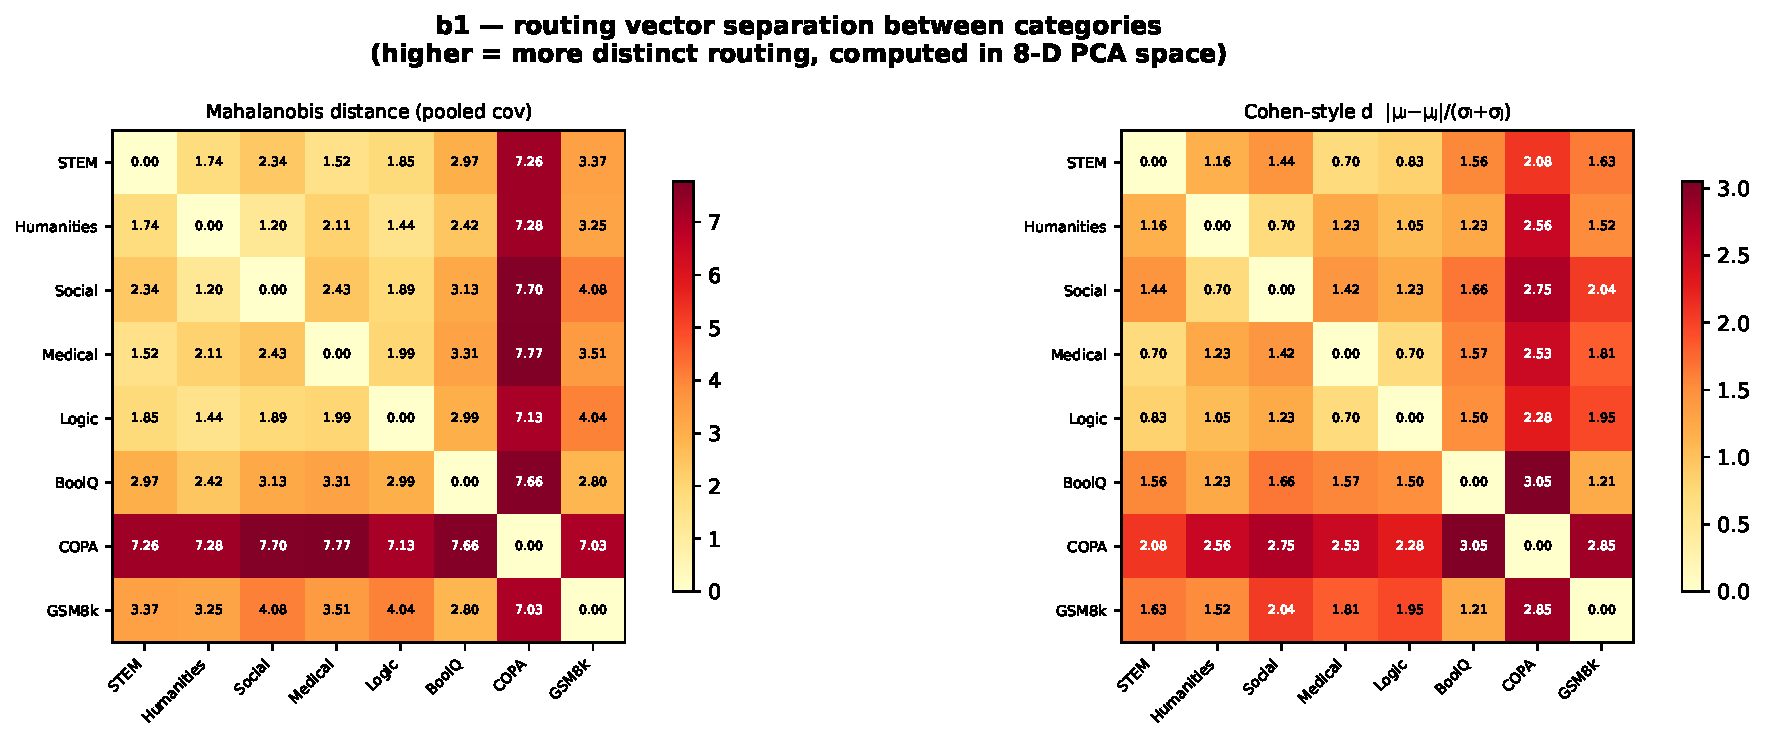
\includegraphics[width=\textwidth]{expert_separation_b1.pdf}
    \caption{B1}
  \end{subfigure}
  \hfill
  \begin{subfigure}[t]{0.48\textwidth}
    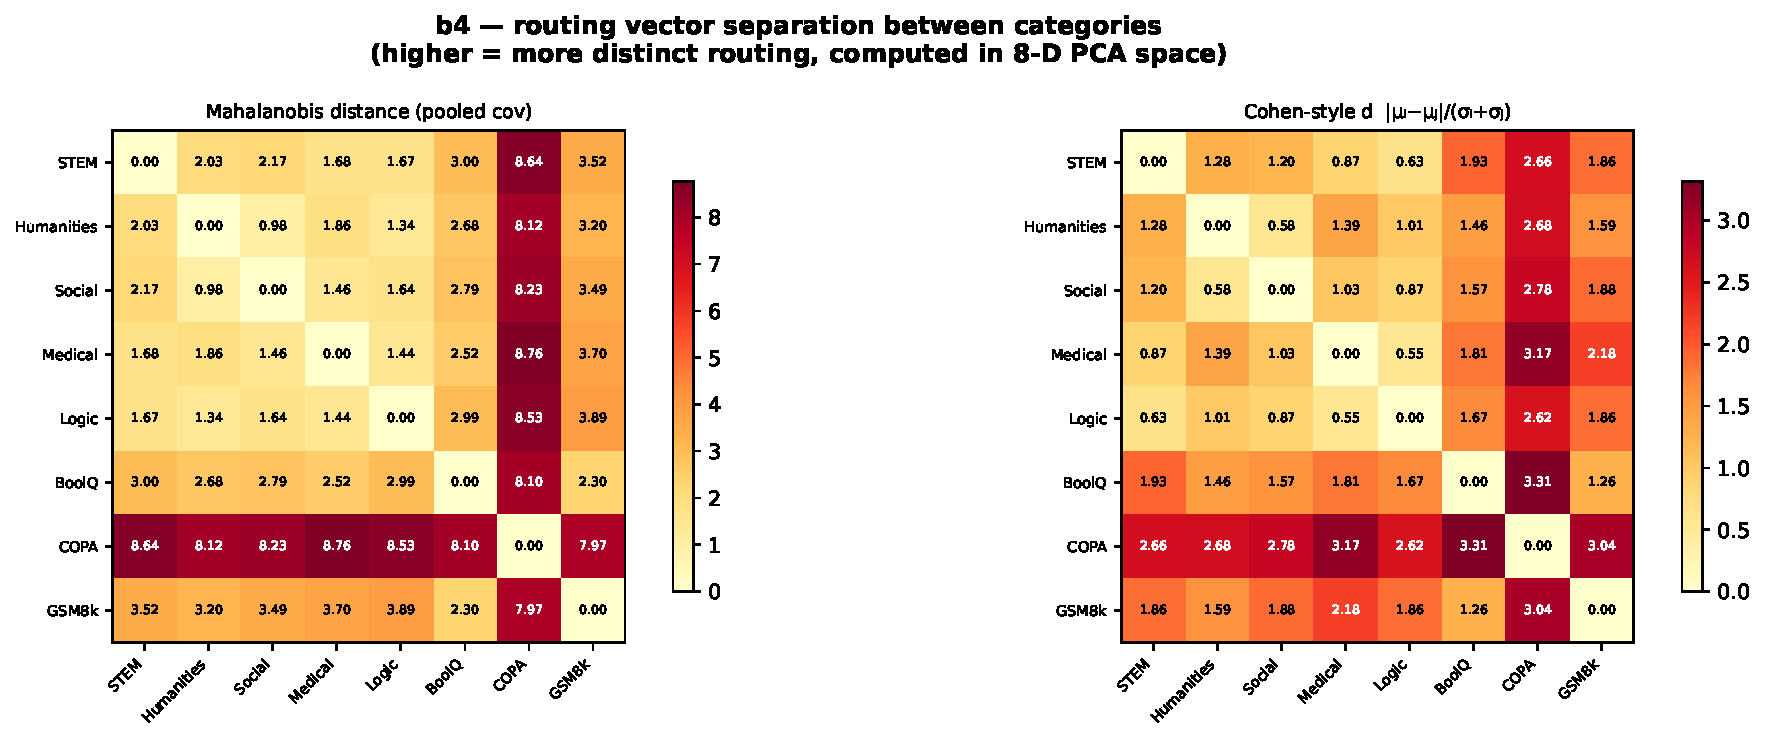
\includegraphics[width=\textwidth]{expert_separation_b4.pdf}
    \caption{B4 (rep\,0.1)}
  \end{subfigure}
  \caption{Pairwise separation heatmaps.
    Left: Mahalanobis distance (pooled covariance).
    Right: Cohen-style $d = \|\mu_i{-}\mu_j\|/(\sigma_i{+}\sigma_j)$.
    COPA is visually isolated in both metrics and both models.}
  \label{fig:separation}
\end{figure}

%% ============================================================
\section{Discussion}
%% ============================================================

\paragraph{Has anything collapsed?}
Partially.  The Boltzmann routing \emph{has} developed hard per-token
assignment ($\hat{K}{\approx}1$ by step~500) and \emph{has} specialised
semantically (2--3 experts cover all input types consistently).
However, only 2--3 of 16 experts are ever used, meaning 13--14 experts
contribute negligibly.  This is a \emph{capacity collapse}: the model
is functioning as a 2--3-expert MoE despite having 16.

\paragraph{Does repulsion help?}
Yes, modestly.  $\lambda{=}0.1$ (B4) reduces max expert load from 0.43 to 0.39
at comparable training steps, with no LM loss penalty.  It does not increase
the number of active experts (still 2--3) but makes the existing routing more
balanced.  $\lambda{=}0.01$ (B2) has a smaller but consistent effect.

\paragraph{Does dropout+WD help?}
No.  Both B3 and B5 show worse load balance and PPL than their repulsion-only
counterparts.  High WD drives all expert weights toward zero but the dominant
expert's gradient signal is largest, so it recovers faster, amplifying the imbalance.

\paragraph{What would work better?}
Direct per-token entropy regularisation
$-\lambda_H\,\mathbb{E}_h[\mathcal{H}(p(\cdot|h))]$ would directly penalise
hard routing.  Alternatively, a load-balancing loss (as in Switch Transformer)
explicitly equalises $\ell_\text{max}$ across experts.

%% ============================================================
\section{Pending results}
%% ============================================================

Table~\ref{tab:benchmarks} will be updated with B2/B3/B4 benchmark results
once eval jobs 74698, 74781, 74701 complete (${\sim}30$--$60$ min).

\end{document}
